\documentclass[11pt]{article}
\usepackage{icmlko}
\begin{document}

\title{미리 적은 거부가 켜졌고, 그 검사가 틀렸다 --- 연도를 안 맞춘 비교에 관하여}
\author{월드모델 실험실}
\date{노트 353 · 2026년 8월 1일}
\maketitle

\begin{abstract}
노트 352가 지목한 것을 했다 --- 아이돌 유보를 $25\to51$ 로 늘렸다(노트
326에서 버려 둔 비한터 2025년 이후 26행). \textbf{구간 폭은 예측대로
$0.757\to0.556$ 으로 줄었다}($1/\sqrt2$). 그런데 같이 미리 적어 둔
\emph{거부 조건}이 켜졌다: 새 26행의 $\rho$ 가 $+0.0972$ 로 한터 25행의
$+0.5188$ 과 0.42 벌어졌다(문턱 0.25). 규약대로면 안 넣는다.
\textbf{갈랐더니 그 검사가 틀린 검사였다.} 아이돌 $\rho$ 는 연도에 크게
흔들리는데(한터 2025 $+0.3131$ 대 2026 $+0.6727$) 두 집합의 연도 구성이
다르다. 연도를 맞추면 2025에서 한터 $+0.3131$(n=14) 대 추가
$+0.3884$(n=17) 로 \textbf{추가 쪽이 낫고}, 벌어짐은 전부 2026의 스무
행에서 온다. 기제까지 찾았다 --- 2025$\to$2026 에 한터는 라벨과 예측이
\emph{같이} 내려가는데(라벨 $-0.61$) 추가는 라벨만 \emph{올라간다}($+0.49$).
묶었을 때 갈리는 것은 실력이 아니라 \textbf{연도 사이 수준}이다. 넣었다.
넣으면 아이돌이 $0.4860\to0.2805$, 판이 $0.4953\to0.4877$ 로
\textbf{내려간다} --- 점수를 보고 고른 것이 아니라는 증거다. 대신 못
가리는 쌍이 $37\to35$ 로 준다.
\end{abstract}

\section{한 일}

노트 326이 아이돌을 넓히면서 규칙을 하나 지켰다 --- ``유보는 안 건드린다''
(노트 82 · 90의 분모 규칙). 추가된 94행 중 2025년 이후 26행을 버리고
학습만 $54\to122$ 로 늘렸다. 판 분모가 그대로여야 옛 점수와 견줄 수 있어서다.

노트 352가 그 대가를 처음 쟀다. 아이돌 $\rho$ 의 95\% 구간이
$[0.052,\,0.817]$ --- 폭 0.756 이다. 판 열 도메인 중 제일 안 재진다.
버린 26행을 넣으면 폭이 $1/\sqrt2$ 로 준다.

\textbf{이 처치에는 재적합이 없다.} 26행은 2025년 이후라 어차피 학습에
안 들어간다 --- ``넣는다''가 바꾸는 것은 \emph{채점 집합}뿐이다. 그래서
모형이 같고, 옛 값과 새 값의 차는 전부 측정에서 온다.

\begin{center}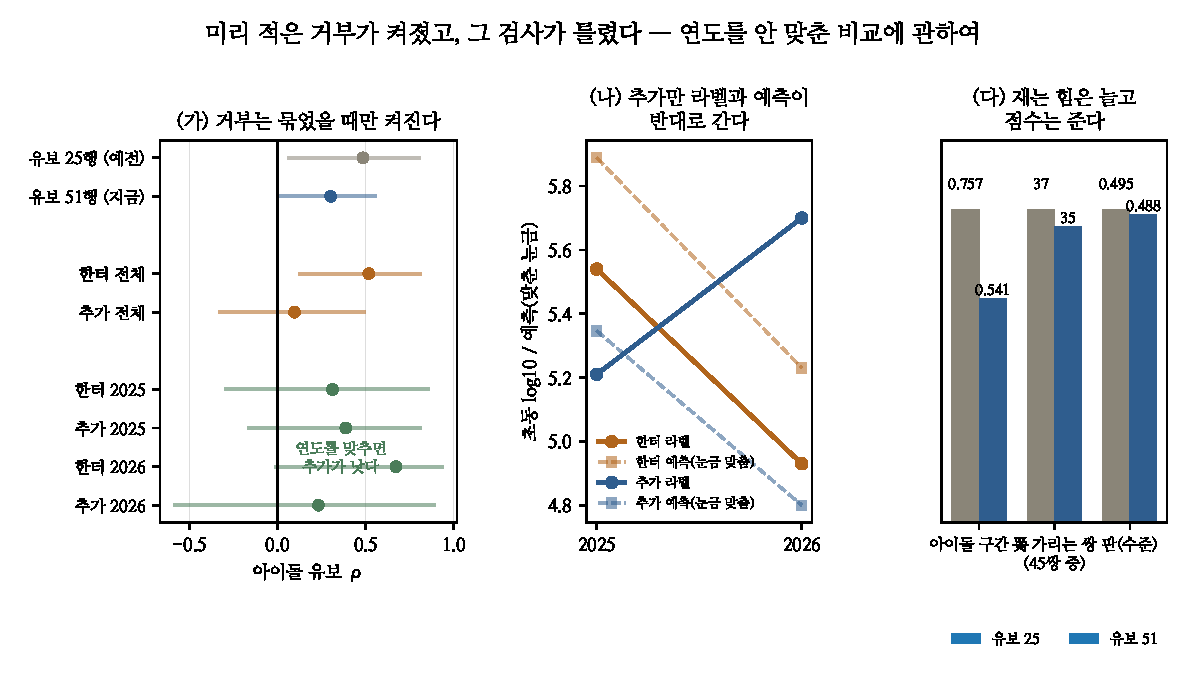
\includegraphics[width=\linewidth]{figs/prereg.pdf}\end{center}

\section{거부가 켜졌다}

미리 적어 둔 조건은 이랬다.

\begin{quote}
새 26행만의 $\rho$ 가 한터 25행과 크게 다르면(차 0.25 이상) 두 라벨
출처가 서로 안 바뀐다는 뜻이고, 폭이 줄어도 \emph{다른 것을 재는 것}이다.
그때는 안 넣는다.
\end{quote}

켜졌다 --- 추가 $+0.0972$, 한터 $+0.5188$, 차 0.42 다.

\section{그런데 그 검사가 틀렸다}

노트 133 이후 규약은 ``첫 수치를 그대로 채택하지 않는다''이고, 그것은
거부 쪽에도 걸린다. 갈랐다.

\begin{center}
\begin{tabular}{lrrl}
\hline
칸 & $n$ & $\rho$ & 95\% 구간 \\
\hline
한터 2025 & 14 & $+0.3131$ & $[-0.300,\,0.861]$ \\
추가 2025 & 17 & $+0.3884$ & $[-0.167,\,0.818]$ \\
한터 2026 & 11 & $+0.6727$ & $[-0.014,\,0.942]$ \\
추가 2026 &  9 & $+0.2333$ & $[-0.590,\,0.895]$ \\
\hline
한터 전체 & 25 & $+0.5188$ & $[+0.118,\,0.821]$ \\
추가 전체 & 26 & $+0.0972$ & $[-0.334,\,0.499]$ \\
\hline
\end{tabular}
\end{center}

\textbf{연도를 맞추면 뒤집힌다.} 행이 제일 많은 2025 칸에서 추가
$+0.3884$ 가 한터 $+0.3131$ 보다 낫다. 벌어짐은 2026의 스무 행에서만
온다. 그리고 아이돌 $\rho$ 는 연도에 크게 흔들린다 --- 한터만 봐도
2025 $+0.31$ 에서 2026 $+0.67$ 이다. \textbf{두 집합의 연도 구성이
다른데 연도를 안 맞추고 견준 것이 검사의 잘못이다.}

\textbf{기제.} 두 전체 값이 제 칸들과 어긋나는 방향이 반대다 --- 한터는
묶으면 오르고($+0.52 >$ 두 칸 다) 추가는 묶으면 내린다($+0.10 <$ 두 칸 다).
연도 사이 수준을 보면 이유가 보인다.

\begin{center}
\begin{tabular}{lrrr}
\hline
 & 라벨 중앙 2025$\to$2026 & 예측 중앙 & 방향 \\
\hline
한터 & $5.54 \to 4.93$ ($-0.61$) & 내려감 & \textbf{같다} \\
추가 & $5.21 \to 5.70$ ($+0.49$) & 내려감 & \textbf{반대} \\
\hline
\end{tabular}
\end{center}

한터는 2026 데뷔가 실제로 초동이 작고 모형도 작게 본다 --- 묶으면 연도
사이 순위가 더 붙는다. 추가는 2026 쪽 라벨이 오히려 크다. 초동 기준이
\texttt{unknown}(20건) · \texttt{ambiguous}(6건) 인 레코드라 \emph{보고
수준}이 연도별로 다를 수 있다. \textbf{묶었을 때 갈리는 것은 실력이 아니라
연도 사이 수준이다.}

\textbf{그리고 애초에 유의하지도 않았다.} 한터 전체 $[+0.118,\,0.821]$ 과
추가 전체 $[-0.334,\,0.499]$ 는 $[0.118,\,0.499]$ 에서 겹친다. 노트 352의
교훈이 이 결정에도 그대로 걸린다 --- 25행과 26행의 차는 못 가린다.

\section{그래서 넣었다 --- 그리고 점수는 내려간다}

\begin{center}
\begin{tabular}{lrr}
\hline
 & 유보 25 & 유보 51 \\
\hline
아이돌 $\rho$      & $0.4860$ & $\mathbf{0.2805}$ \\
아이돌 구간 폭     & $0.757$  & $\mathbf{0.541}$ \\
판                 & $0.4953$ & $\mathbf{0.4877}$ \\
판 분모            & 2,669    & 2,695 \\
못 가리는 쌍(45 중)& 37       & $\mathbf{35}$ \\
\hline
\end{tabular}
\end{center}

\textbf{점수로 고른 것이 아니라는 증거는 방향이다.} 넣으면 아이돌이
0.21 내려가고 판이 0.008 내려간다. 분모가 바뀌니 옛 판 수와 직접 견줄
수도 없다. 얻은 것은 하나뿐이다 --- \emph{재는 힘}. 구간 폭이 0.22 줄고
순서를 가릴 수 있는 쌍이 둘 늘었다.

\textbf{그리고 이것이 노트 352의 규약이 시키는 일이다.} ``낮아 보이는
도메인을 쫓지 말고 짝으로 오르는 처치를 쫓는다''는 반대로도 읽힌다 ---
\emph{높아 보이는 수를 지키려고 못 재는 상태를 유지하지 않는다.} 아이돌
0.486 은 유보 25행이 준 낙관이었다.

\section{규약을 고친다}

\begin{itemize}
\item \textbf{부분집합을 견줄 때는 연도를 맞춘다.} 이 판의 $\rho$ 는
연도에 크게 흔들린다(아이돌 한터 $+0.31 \to +0.67$). 연도 구성이 다른
두 집합을 묶어서 견주면 실력 차가 아니라 연도 차를 본다. 노트 353의
거부 조건이 그 함정에 그대로 빠졌다.
\item \textbf{미리 적은 거부를 뒤집을 때는 기제까지 보인다.} 여기서는
연도 맞춤 + 수준 방향 + 구간 겹침 셋을 다 적었다. 셋 없이 뒤집으면
그냥 점수 고르기다.
\item \textbf{자료 결정은 점수 방향으로 검산한다.} 이 결정은 점수를
내린다 --- 그래서 안전하다. 점수를 올리는 자료 결정은 같은 증거로도
더 의심해야 한다.
\end{itemize}

\section{남은 것}

\begin{center}
\begin{tabular}{ll}
\hline
갈래 & 지금 아는 것 \\
\hline
추가 2026 아홉 행 & 라벨 수준이 한터와 반대. \texttt{unknown} 기준 20건을 \\
                  & 확인하면 수준 보정이 가능할 수 있다 \\
시장팝업 유보 늘리기 & 미채택 542건. 폭 $0.400\to0.283$ \\
등급이 왜 거꾸로인가 & 노트 352에서 설명 셋 실패. 열어 둔다 \\
검사 ⑤ 를 규약에 & ③ 뒤에만(노트 351) \\
\hline
\end{tabular}
\end{center}

첫 줄이 다음이다. 아홉 행짜리 사실이지만 그 아홉 행이 아이돌 유보의
18\%다.

\end{document}
